% Multi-Head Attention - Diagrama de flujo
% Compilar con: pdflatex multi_head_attention.tex
\documentclass[tikz,border=10pt]{standalone}
\usepackage{tikz}
\usepackage{amsmath,amssymb}
\usetikzlibrary{arrows.meta, positioning, calc, fit}

\definecolor{gdlblue}{RGB}{41, 98, 168}
\definecolor{gdlred}{RGB}{191, 49, 49}
\definecolor{gdlgreen}{RGB}{30, 130, 76}
\definecolor{gdlorange}{RGB}{217, 130, 30}
\definecolor{gdlpurple}{RGB}{118, 56, 138}
\definecolor{gdlgray}{RGB}{140, 140, 140}
\definecolor{gdlyellow}{RGB}{190, 140, 10}

\begin{document}
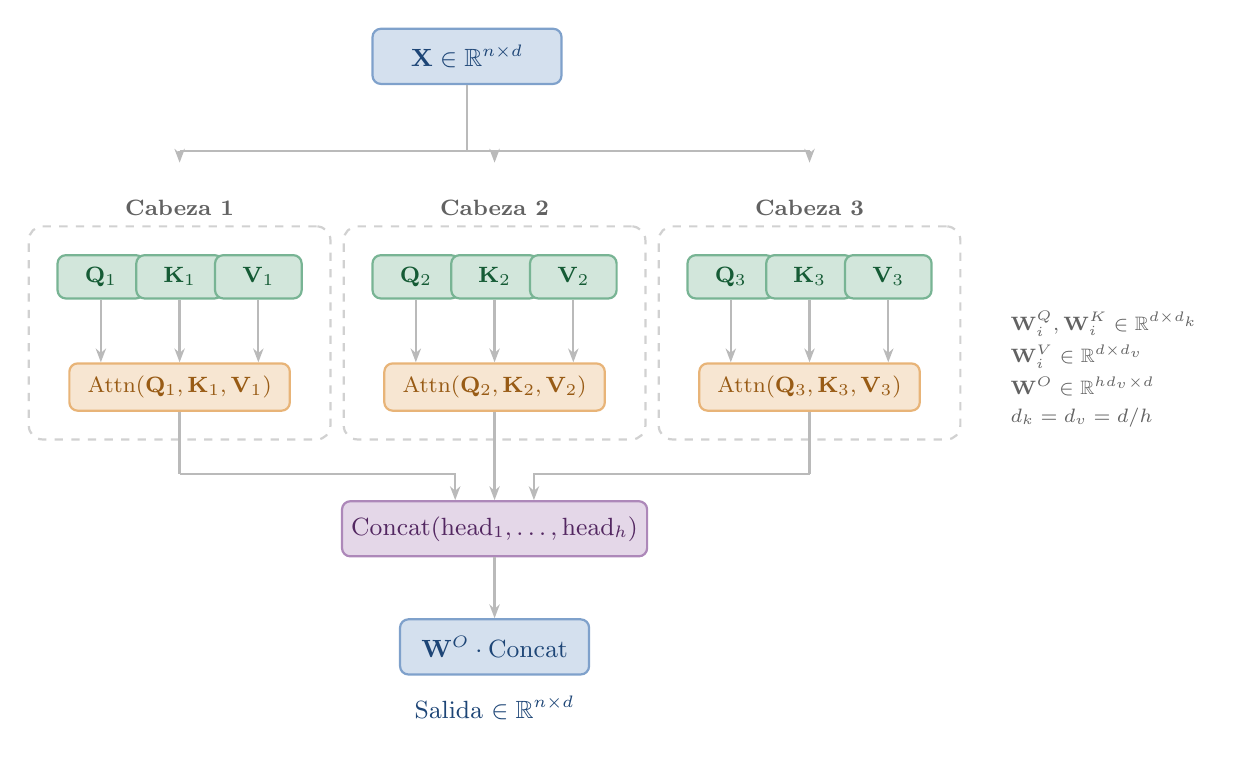
\begin{tikzpicture}[
    arrow/.style={-{Stealth[length=5pt]}, thick, draw=gdlgray!60},
    line/.style={thick, draw=gdlgray!60},
    inputbox/.style={rectangle, rounded corners=3pt, draw=gdlblue!60, fill=gdlblue!20,
        thick, minimum width=2.4cm, minimum height=0.7cm, font=\small,
        text=gdlblue!70!black, align=center},
    projbox/.style={rectangle, rounded corners=3pt, draw=gdlgreen!60, fill=gdlgreen!20,
        thick, minimum width=1.1cm, minimum height=0.55cm, font=\footnotesize,
        text=gdlgreen!70!black, align=center},
    attnbox/.style={rectangle, rounded corners=3pt, draw=gdlorange!60, fill=gdlorange!20,
        thick, minimum width=2.8cm, minimum height=0.6cm, font=\footnotesize,
        text=gdlorange!70!black, align=center},
    concatbox/.style={rectangle, rounded corners=3pt, draw=gdlpurple!60, fill=gdlpurple!20,
        thick, minimum width=3.2cm, minimum height=0.7cm, font=\small,
        text=gdlpurple!70!black, align=center},
    outputbox/.style={rectangle, rounded corners=3pt, draw=gdlblue!60, fill=gdlblue!20,
        thick, minimum width=2.4cm, minimum height=0.7cm, font=\small,
        text=gdlblue!70!black, align=center},
    headlabel/.style={font=\footnotesize\bfseries, text=gdlgray!70!black},
    dashedbox/.style={rectangle, rounded corners=5pt, draw=gdlgray!40, dashed,
        thick, inner sep=10pt, inner ysep=10pt}
]

% === Layout constants ===
\def\headspacing{4.0}
\def\projy{-2.8}
\def\attny{-4.2}
\def\distribY{-1.2}
\def\concaty{-6.0}
\def\outputy{-7.5}

% === Input ===
\node[inputbox] (input) at (0, 0) {$\mathbf{X} \in \mathbb{R}^{n \times d}$};

% === Head 1 (left) ===
\node[projbox] (q1) at ({-\headspacing - 0.65}, \projy) {$\mathbf{Q}_1$};
\node[projbox] (k1) at ({-\headspacing + 0.35}, \projy) {$\mathbf{K}_1$};
\node[projbox] (v1) at ({-\headspacing + 1.35}, \projy) {$\mathbf{V}_1$};
\node[attnbox] (attn1) at ({-\headspacing + 0.35}, \attny)
    {$\mathrm{Attn}(\mathbf{Q}_1, \mathbf{K}_1, \mathbf{V}_1)$};

% === Head 2 (center) ===
\node[projbox] (q2) at ({-0.65}, \projy) {$\mathbf{Q}_2$};
\node[projbox] (k2) at (0.35, \projy) {$\mathbf{K}_2$};
\node[projbox] (v2) at (1.35, \projy) {$\mathbf{V}_2$};
\node[attnbox] (attn2) at (0.35, \attny)
    {$\mathrm{Attn}(\mathbf{Q}_2, \mathbf{K}_2, \mathbf{V}_2)$};

% === Head 3 (right) ===
\node[projbox] (q3) at ({\headspacing - 0.65}, \projy) {$\mathbf{Q}_3$};
\node[projbox] (k3) at ({\headspacing + 0.35}, \projy) {$\mathbf{K}_3$};
\node[projbox] (v3) at ({\headspacing + 1.35}, \projy) {$\mathbf{V}_3$};
\node[attnbox] (attn3) at ({\headspacing + 0.35}, \attny)
    {$\mathrm{Attn}(\mathbf{Q}_3, \mathbf{K}_3, \mathbf{V}_3)$};

% === Arrows: projections -> attention (all heads) ===
\foreach \h in {1,2,3} {
    \draw[arrow] (q\h.south) -- (attn\h.north -| q\h.south);
    \draw[arrow] (k\h.south) -- (attn\h.north -| k\h.south);
    \draw[arrow] (v\h.south) -- (attn\h.north -| v\h.south);
}

% === Dashed boxes around each head ===
\node[dashedbox, fit=(q1)(v1)(attn1)] (hbox1) {};
\node[dashedbox, fit=(q2)(v2)(attn2)] (hbox2) {};
\node[dashedbox, fit=(q3)(v3)(attn3)] (hbox3) {};

% === Head labels (above each dashed box) ===
\node[headlabel, anchor=south] at (hbox1.north) {Cabeza 1};
\node[headlabel, anchor=south] at (hbox2.north) {Cabeza 2};
\node[headlabel, anchor=south] at (hbox3.north) {Cabeza 3};

% === Distribution: input -> horizontal line -> heads ===
% Vertical stem from input
\draw[line] (input.south) -- (0, \distribY);
% Horizontal bar spanning all three heads
\draw[line] ({-\headspacing + 0.35}, \distribY) -- ({\headspacing + 0.35}, \distribY);
% Arrows down from bar to each head (landing above "Cabeza" label)
\pgfmathsetmacro{\arrowEndY}{\projy + 1.45}
\draw[arrow] ({-\headspacing + 0.35}, \distribY) -- ({-\headspacing + 0.35}, \arrowEndY);
\draw[arrow] (0.35, \distribY) -- (0.35, \arrowEndY);
\draw[arrow] ({\headspacing + 0.35}, \distribY) -- ({\headspacing + 0.35}, \arrowEndY);

% === Concatenation ===
\node[concatbox] (concat) at (0.35, \concaty)
    {$\mathrm{Concat}(\mathrm{head}_1, \ldots, \mathrm{head}_h)$};

% Convergence line y-coordinate (between attention boxes and concat)
\pgfmathsetmacro{\convY}{\concaty + 0.7}

% Arrows from attention outputs converging into concat
% Head 1: down, right along convergence line, into concat left
\draw[line] (attn1.south) -- (attn1.south |- 0, \convY);
\draw[arrow] (attn1.south |- 0, \convY) -| ($(concat.north) + (-0.5, 0)$);
% Head 2: straight down
\draw[arrow] (attn2.south) -- (concat.north);
% Head 3: down, left along convergence line, into concat right
\draw[line] (attn3.south) -- (attn3.south |- 0, \convY);
\draw[arrow] (attn3.south |- 0, \convY) -| ($(concat.north) + (0.5, 0)$);

% === Final linear projection ===
\node[outputbox] (output) at (0.35, \outputy)
    {$\mathbf{W}^O \cdot \mathrm{Concat}$};
\draw[arrow] (concat.south) -- (output.north);

% === Output label ===
\node[font=\small, text=gdlblue!70!black, below=4pt of output]
    {Salida $\in \mathbb{R}^{n \times d}$};

% === Annotation: weight dimensions (right margin) ===
\node[font=\scriptsize, text=gdlgray!70!black, align=left, anchor=north west]
    at ($(hbox3.east) + (0.5, 0.4)$)
    {$\mathbf{W}_i^Q, \mathbf{W}_i^K \in \mathbb{R}^{d \times d_k}$\\[2pt]
     $\mathbf{W}_i^V \in \mathbb{R}^{d \times d_v}$\\[2pt]
     $\mathbf{W}^O \in \mathbb{R}^{hd_v \times d}$\\[2pt]
     $d_k = d_v = d/h$};

\end{tikzpicture}
\end{document}
